\chapter{Evaluierung}
\label{ch:S6_Evaluierung}

\section{Qualität der Lösung}
\label{ch:CH6_qualtiy_of_solution}

Für eine Evaluation der in Kapitel \ref{ch:S4_Lösungsansatz} und \ref{ch:S5_Umsetzung} vorgestellten Lösung muss zunächst die Evaluationsmethode definiert werden. Für die Evaluation soll die Lösung mit der in Kapitel \ref{ch2:Problemstellunug} definierten Problemstellung gegenübergestellt werden. Es wird daher untersucht, inwiefern das Framework, sowie das Beispielspiel zur einer Lösung der Problemstellung beitragen. Das Ergebnis der Evaluation soll entsprechend weitere Handlungsempfehlungen bzw. Verbesserungsvorschläge aufzeigen, sofern diese aufgrund der Evaluation notwendig sein sollten. 
Zunächst sollen die nachfolgenden Punkte analysiert werden im Hinblick auf die dargestellte Lösung:

\begin{itemize}

\item Gamification unter Einbezug der Händler
\item Pervasive Games
\item Relokalisierbarkeit
\item Verwendbarkeit von OSM Daten

\end{itemize}

Die Evaluation der Spielfelder, welche durch das Framework erzeugt werden und somit eine Bewertung der Relokalisierbarkeit wurde als eigenständiger Part in Kapitel \ref{ch:CH6_qualtiy_of_gameboards} separat behandelt.


\subsection*{Gamification}

Im Bezug auf die in Kapitel \ref{ch1:Einleitung} aufgestellte Forschungsfrage soll die Lösung mittels Gamification den regionalen Händlern zu neuen Kunden führen können und bestehende entsprechend halten. Ziel ist es nicht zu überprüfen, ob und wie hoch der entsprechende Neukunden und Bestandskundenanteil durch die Lösung beeinflusst wird, sondern inwiefern entsprechende Elemente aus der Literatur umgestzt wurden. Diese wiederum sollen die Möglichkeit für einen besseren Umsatz der Händler bieten.
In der Literatur wurden zunächst die rudimentären Elemente eines Gamification Prozesses herauskristalisiert. Für die softwaretechnische Umsetzung wurden entsprechende Möglichkeiten geschaffen und entsprechend integriert, damit die typischen Elemente Points, Badges und Leaderboards problemlos über umgesetzt werden können. Zudem wurden die Aspekte der klassischen Spieltheorie aufgegriffen und dadurch die Gamificationen Ansätze erweitert. Es wurden mehreren Optionen aufgezeigt, welche in Spielen umgesetzt werden können. Darüber hinaus wurden diese Aspekte mit entsprechenden Technologien wie NFC, oder Bluetooth Low Energy in Verbindung gebracht, wie eine Integration der Spielelemente vor Ort bei den Händlern gestaltet werden könnte. Das Framework und das Beispielspiel bilden diese nich talle ab, sind aber entsprechend in diese Richtung problemlos erweiterbar.
Durch eine entsprechende Kombination der Gamification Elemente und der Tatsache, dass das Framework auf Basis von Informationen aus der Umgebung Spielelemente aufbereitet und lokale Händler integriert wird auch das Maß der Immersion entsprechend für die Spieler erhöht und der Effekt der Gamification verstärkt.
Für den Aspekt der Gamification lässt sich daher abschließend festhalten, dass die aufgezeigte Lösung einen Beitrag zur Lösung der Problematik der Gamification von Neukundenbesuchen bei regionalen Händlern liefern kann.

\subsection*{Pervasive Games  - Anforderungen an ein Gameframework}

Im Zuge der Erstellung eines Frameworks zum Staging von Pervasive Games müssen mehrere Aspekte behandelt werden. Zunächst muss sichergestellt werden, dass die definierten Grenzen des Magic Circle überschritten werden können. Im Zuge dieser Arbeit ging es darum die Dimension Ort und Zeit zu lösen. Das bedeutet, dass Spiel soll sowohl ortsunabhängig als auch zeitunabhängig gespielt werden kann. Die Ortsunabhängigkeit der vorgestellten Lösung wird durch die Relokalisierung mit Hilfe von OSM-Daten sichergestellt, auf die später im Detail eingegangen wird. Die zeitliche Unabhängigkeit ist dadurch sichergestellt, dass jeder Spieler sich individuell am Beispielspiel anmelden kann und es keine fest definierten Uhrzeiten oder Termine gibt um das Spiel zu spielen. Im Vergleich zu typischen Geogames ist es daher möglich auch über feste Uhrzeiten und Geografische Gebiete hinaus das Spiel zu spielen. Durch die entsprechende Formulierung der Anforderungen in Kapitel \ref{ch2:Problemstellunug} und \ref{ch4:s:Lösungen} und der Ausrichtung des Frameworks an diesen wurde sichergestellt, dass das Framework diese Anforderungen erfüllt. Da es sich in der Problemstellung um ein Echzeitspiel handelt muss auch entsprechend im Framework sichergestellt werden, dass die Interaktion mit dem Spiel in Echtzeit erfolgen kann.
Durch die Modularisierung und Auskopplung der Evaluation der OSM Tags, ist es möglich geworden die zeitintensiven Bewertungs-Funktionalitäten unabhängig von der Spielfeldgenerierung durchzuführen. Dadurch ist wird es ermöglicht, lediglich die relativ einfachen Prozesse zur Transformation der OSM-Elemente während der Laufzeit durchzuführen. Vergleicht man die Antwortzeit der Requests , welche abhängig sind von der Anzahl der OSM-Elemente in der Bouding Box und der Antwortzeit des Overpass API Servers, so liegen diese im Schnitt bei ca. 400ms. Die Varianz ist wie in Abbildung \ref{img:ch6_img01_response_time} erkenntlich zu vernachlässigen. Die Evaluationsfunktion hingegen liegt bei 2-3 Minuten für ein Tag mit ca. 200 Elementen. Für ein Feld mit 1200 Elementen liegt diese bereits bei über 30 Minuten.

\begin{figure}[H]
\begin{center}
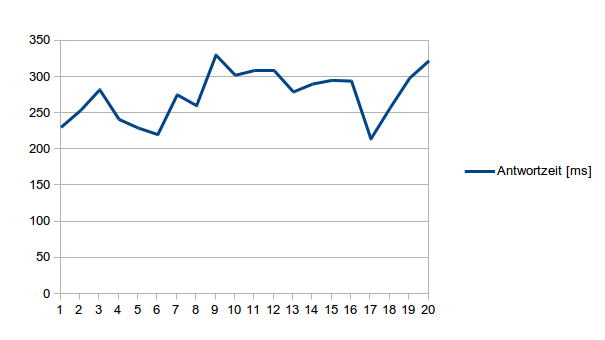
\includegraphics[width=150mm]{images/ch6_img01_response_time.png}
\caption{Antwortzeit der GameAPI für den Tag public\_transport=stop\_area}
\label{img:ch6_img01_response_time}
\end{center}
\end{figure}

Abweichungen der Antwortzeit sind weniger bedeutend, da das Spielfeld sich bereits vorher für den Spieler aufbaut und die Spielelemente mittels Ajax Request geladen werden. Darüber hinaus wird durch die dynamische Erweiterung der Bounding Box sichergestellt, dass alle Elemente am Rand der Karte bereits geladen sind. Das Nachladen der Elemente beim Fortbewegen kann daher auch minimal länger dauern, da das Spielfeld immer zentriert auf den Spieler ist.

Durch die Kapselung der einzelnen Module wird auch sichergestellt, dass eine Erweiterbarkeit der Spielmechnaik ohne größeren Aufwand möglich ist. Das entsprechende Beispielspiel kann problemlos erweitert werden oder aber durch ein beliebiges anderes Spiel ersetzt werden.
Hierbei zeigt sich, dass die Anforderung für die Flexibilität des Frameworks hinsichtlich seiner Erweiterbarkeit und Austauschbarkeit gegeben ist.

\subsection*{Relokalisierbarkeit}

Der nächste essentielle Aspekt der Problemstellung war die Relokalisierbarkeit. Ziel war es im Zuge des zu vereinfachenden Stagings dem Spielleiter entsprechend eine Möglichkeit an die Hand zu geben, welche im auch ein Spielen außerhalb eines festen Bereiches ermöglicht. Hierzu wurden entsprechende OSM-Daten verwendet die durch eine Transformation zu Spielelementen umgewandelt wurden. Durch die entsprechende Evaluation der OSM-Tags im Voraus wird sichergestellt, dass der jeweils beste Tag für die getesteten Umgebungen ausgewählt wurde.
Die Transformation der OSM-Elemente funktioniert problemlos, speziell auch mit Relationen und Ways, wie in Abbildung \ref{img:ch6_img02_transform} zu erkennen ist. Auf der linken Seite sind die Daten aus OSM respektive Overpass zu sehen. Auf der rechten Seite sind hingegen die vom Framework erzeugen Spielelemente ersichtlich.


\begin{figure}[H]
\begin{center}
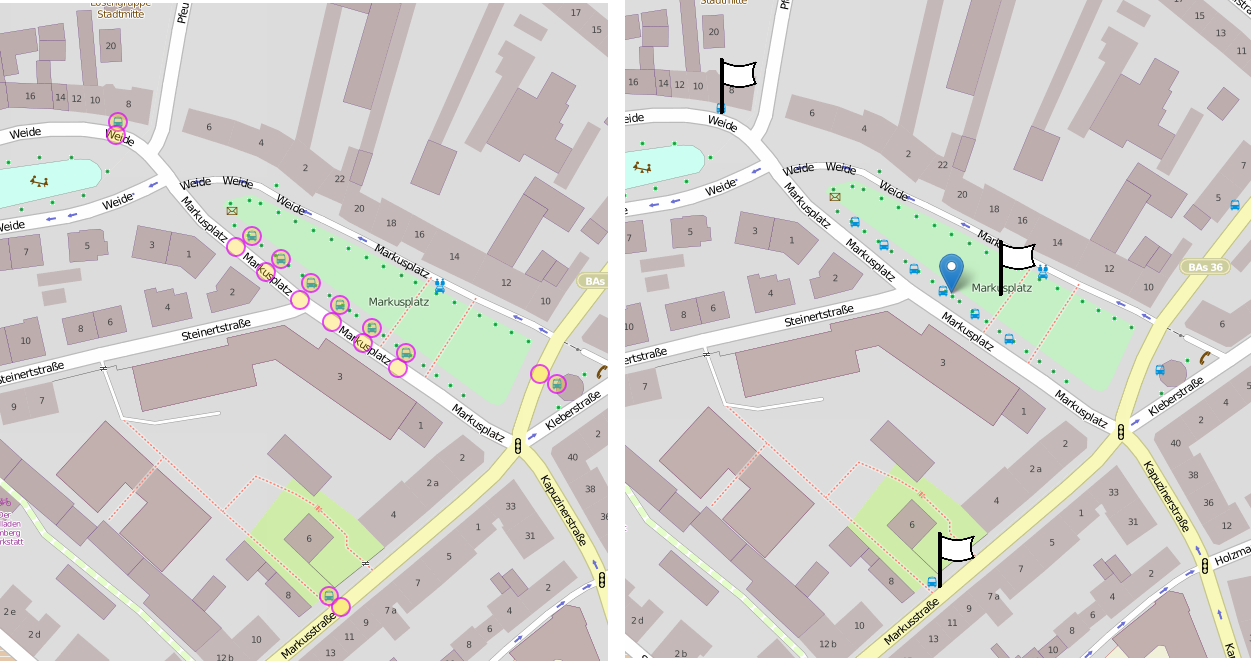
\includegraphics[width=150mm]{images/ch6_img02_transform.png}
\caption{OSM-Daten im Vergleich zu den transformierten Spielelementen}
\label{img:ch6_img02_transform}
\end{center}
\end{figure}

Sofern eine entsprechende Evaluierung sichergestellt wurde im Voraus, sind die Spielfelder entsprechend nutzbar.
Einen Nachteil der die Fokusierung auf ein einzelnes Key-Value Paar in OSM mit sich bringt, ist die Möglichkeit, dass es z.B. in Regionen in denen eine geringere Mapping Qualität vorliegt, im Extremfall keine Spielelemente zur Verfügung stehen könnten. Diese Problematik könnte in dem Fall durch eine einfache Anpassung des Frameworks gelöst werden. Hierzu müsste intern eine Liste vorgehalten werden mit alternativen Tags. Diese Liste könnte auch dynamisch auf Basis von \url{http://taginfo.openstreetmap.ch/tags} gefüllt werden. Beim Request müsste das Framework nur die vorhandene Zahl der Spielelemente prüfen und bei einer Unterschreitung eines vordefinierten Wertes automatisch der nächste alternative Tag verwendet werden. Zwar führt das dazu, dass potentiell die Auswahl der Spielelemente für den Spieler schwerer nachvollziehbar ist, jedoch würde dies sicherstellen, dass auch im Worst Case Szenario entsprechende Spielelemente generiert werden.

Somit lässt sich feststellen, dass die Relokalisierung problemlos funktioniert und auch entsprechend für den Einsatz mit Pervsaive Games geeignet ist. Ein offener Punkt ist eine weitere Optimierung für das Worst Case Szenario für den Fall, dass der optimale Tag im lokalen Bereich keine Spielfelder liefern kann.

\subsection*{Verwendbarkeit von OSM Daten}

Eine Fragestellung zu Beginn der Arbeit war die Verwendbarkeit von OSM Daten im Zuge von Pervasive Games.
Die Anforderungen an die Daten im Vergleich zu einer Navigationssoftware sind beim Framework vergleichsweise gering.
Es muss eine korrekte Klassifikation stattfinden und die Abweichung der Position sollte vorzugsweise nicht mehr als der Aktionsradius des Spielers betragen. Dadurch wird erreicht, dass alle Spielelemente auch entsprechend von den Spielern physikalisch erreichbar sind.
Fehler bei der Klassifikation können vorkommen, da es immer der Fall sein kann, dass die Daten nicht entsprechend korrekt gemappt wurden.
Dies ist aber im Zusammenhang des Frameworks nicht weiter tragisch, da deswegen maximal das entsprechende Element/Objekt nicht auf dem Spielfeld erscheinen wird. Dadurch wird aber die Funktionalität des jeweiligen Spieles selbst nicht berührt. Hierdurch wird lediglich die Verteilung auf dem Spielfeld beeinflusst. Probleme mit dem Spielfeld bei zu wenig Elementen wurden bereits angesprochen und mögliche Lösungen aufgezeigt.
Die Transformation der OSM-Daten wurde so vorgenommen, dass auch bei Mapping Fehlern, z.B. das rekursive Verweisen von Relations, keine Probleme verursachen. Es wird sichergestellt, dass in jedem Fall die Transformation stattfindet.
Dadurch, dass die Ergebnisse in der Literatur OSM eine ausreichende Datenqualität zusprechen und OSM auch für kommerzielle Produkte verwendet wird und bei allen Tests mit dem Gameframework gute Ergebnisse lieferte ist abschließend festzuhalten, dass OSM ohne Einschränkungen nutzbar ist.

\subsection*{Abschließendes Ergebnis}

Für den Spielleiter lässt sich daher festhalten, dass die Anforderungen für ein einfaches Staging erfüllt werden. Darüberhinaus findet auch die geforderte Modularisierung der einzelne Funktionen statt. Die einzelnen Komponenten ermöglichen es mithilfe von OSM-Daten entsprechende Spiefelder zu erzeugen, welche unter Einbindung der virtuellen Händler und entsprechender Gamification Elemente des Beispielspiels zu einer Lösung der in Kapitel XX vorgestellten Probleme führt.


\section{Qualität der Spielfelder}
\label{ch:CH6_qualtiy_of_gameboards}

-qualität der spielfelder

-idealfall 2D: fläche mit punkten gleicher abstand

-aber bewegung nur auf wegen möglich

--> zu komplexes problem

--> evaluation der abstände notwendig zwischen den Spielelementen

-verwendung OSM

-offline routing

-inner und outter bounding box

-Zeigraphisches Netzwerk (Fußweg 10min)

ist punkt auf Netzwerk?

--> zu langsam

--> direktes routing ---> graphopper

-kNN bzw. cNN

-harte abgernzung unvorteilhaft

--> zeitgraphisches netzwerk nciht verwendbar

--> bewerteter graph

--> fuzzy, funktion 2. ordnung